\documentclass[12pt,a4paper]{ctexart}
\usepackage{amsmath,amsthm,amssymb,
appendix,bm,graphicx,hyperref,mathrsfs,
abstract,pdfpages}

\linespread{1.5}

%图片路径%
\graphicspath{{./picture/}}
%删除图片后缀名,这样只需要打图片名字即可%
\DeclareGraphicsExtensions{.pdf,.jpeg,.png,.jpg}

%%定理环境
\newtheorem{theorem}{定理}[section]
\newtheorem{definition}[theorem]{定义}
\newtheorem{lemma}[theorem]{引理}		
\newtheorem{corollary}[theorem]{推论}
\newtheorem{example}[theorem]{例}
\newtheorem{proposition}[theorem]{命题}

%%
\renewcommand{\abstractname}{\Large\textbf{摘要}}

\begin{document}

	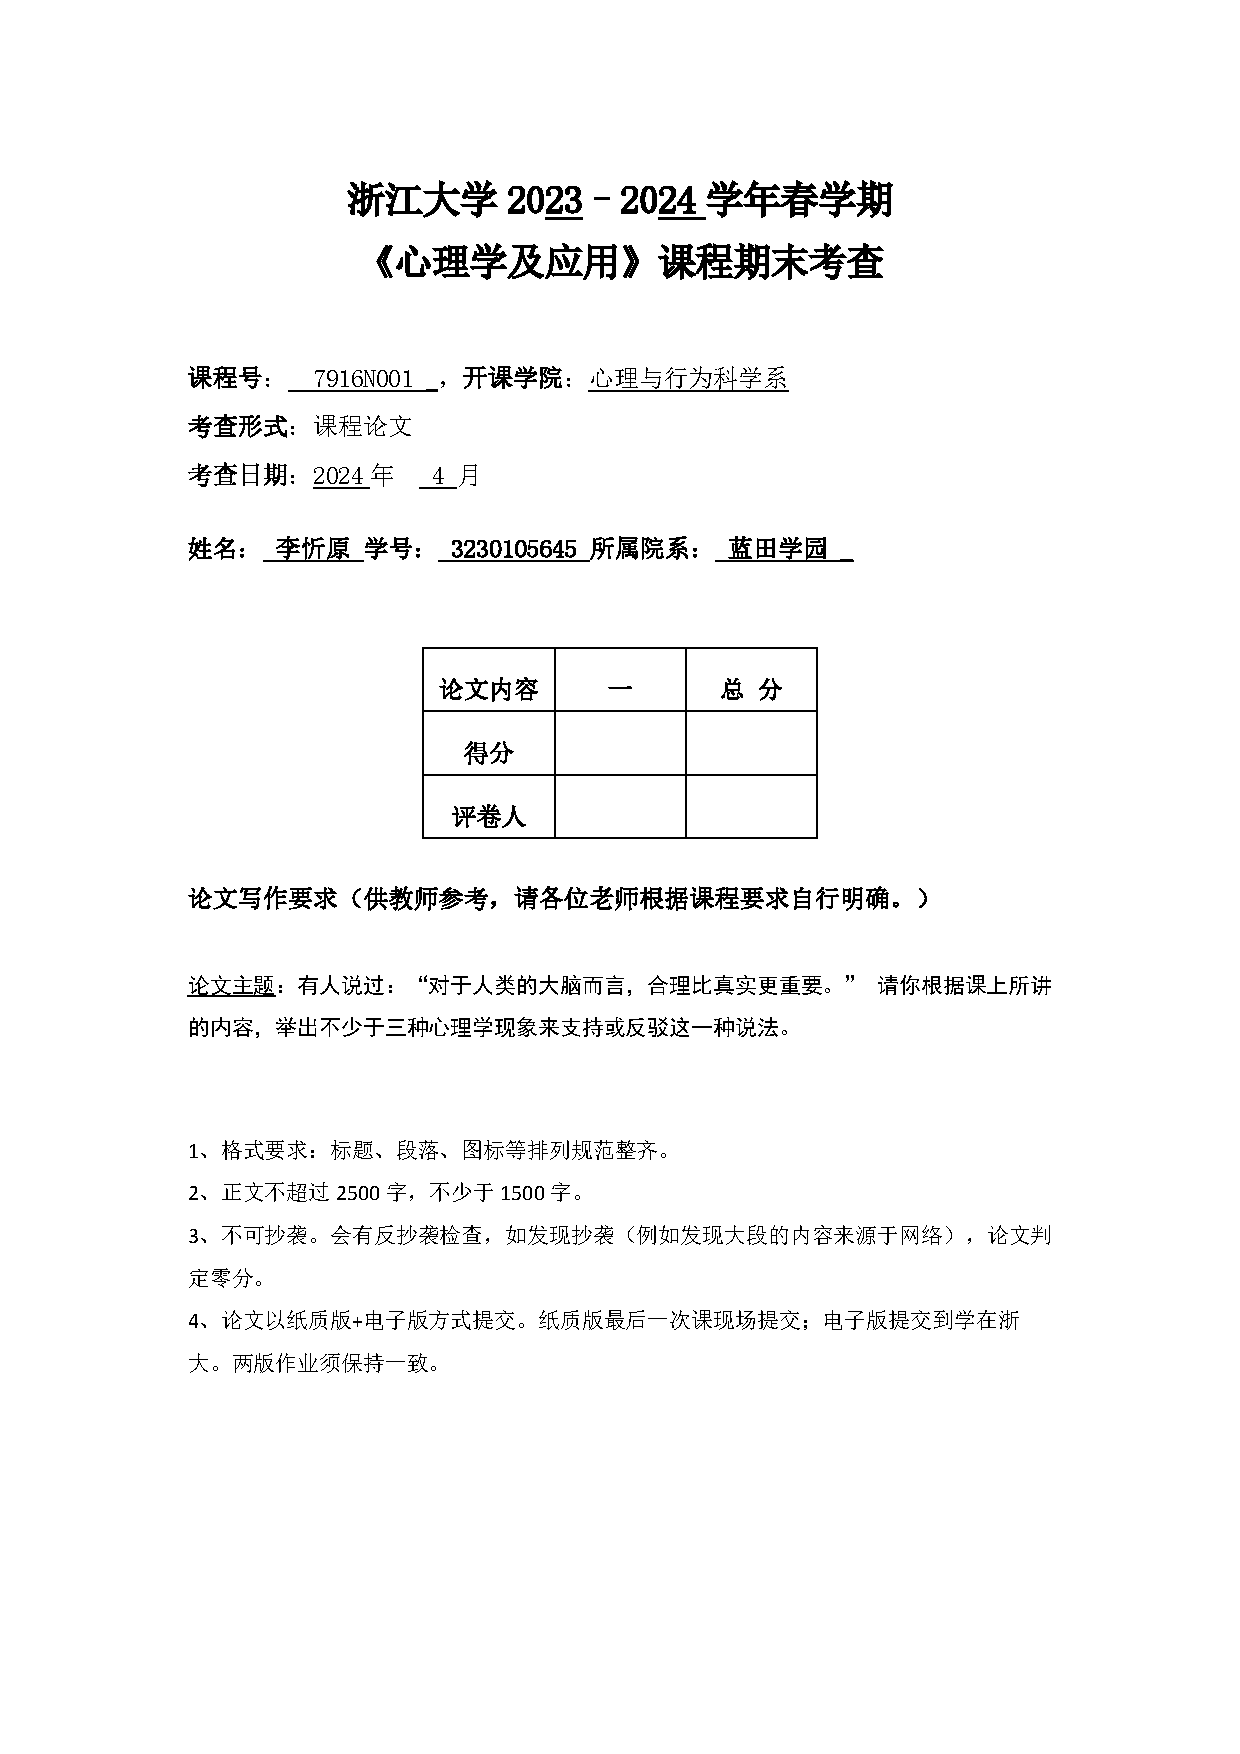
\includepdf{心理学及应用 课程论文封面 .pdf}
	\thispagestyle{empty}
	
	\begin{abstract}
		历来,就“对于人类的大脑而言,合理比真实更重要”
		这一观点众说纷纭。从大脑的结构出发,通过分析其
		感觉及知觉形成过程,以及大脑的思考方式,再结合
		三例具体的心理学现象:Müller-Lyer illusion、
		Beuchet Chair Illusion、
		Dutton \texorpdfstring{\&}{} Aron, 1974 吊桥实验,
		我认为这一观点有其合理性。
		\par\textbf{关键词:}Müller-Lyer illusion; 
		Beuchet Chair Illusion; 
		Dutton \texorpdfstring{\&}{} Aron, 1974 吊桥实验; 
		合理性; 真实性; 感知; 知觉;

	\end{abstract}
	
	
	\newpage
	\section{引言}
	从人类的生理结构上分析,感受器在感受到特征后,通过电刺
	激将兴奋传导到大脑皮层,经过大脑皮层处理后形成知觉。但
	实际上,知觉过程并不是对感觉信号的忠实解读,知觉的结果
	与感觉的物理输入可能有较大的差别。

	我们的大脑首先对输入的基本感觉信息进行抽提,形成简单的
	知觉特征,如颜色、亮度、线条朝向等。然后,我们的大脑再
	通过知识经验,进行合理的推断,即使这种推断可能是以牺牲
	一定真实性为代价的,最终形成知觉。

	接下来,我将分为错觉和情绪两个方面,通过三个实例
	作证这一观点。



	\section{错觉}
	\subsection{定义}
	错觉是指我们感知到的信息与实际情况不一致的现象。它们是我们
	感觉系统的一种特殊表现,经常发生在我们的日常生活中。错觉可
	以涉及各种感官,包括视觉、听觉、触觉、嗅觉和味觉。它们可能
	是由于感官系统的工作方式、神经传递的错误、大脑的解释和理解
	过程等因素引起的。

	在这种错觉中,以视觉错觉为例,大脑会根据我们接收到的一部分
	信息,结合我们以往的经验和知识,自动脑补出“合理”的结果,而
	可能与真实情况相悖。以下将通过两例分析。

	\subsection{缪勒-莱尔错觉(Müller-Lyer illusion)}
	缪勒-莱尔错觉(Müller-Lyer illusion)是一种视觉错觉,最早
	由德国心理学家缪勒(Franz Carl Müller-Lyer)于1889年发现。
	这个错觉是通过两条等长的直线段,但它们的末端有不同的箭头或
	者短横线装饰而产生的。
	\begin{figure}[h]
		\centering
    	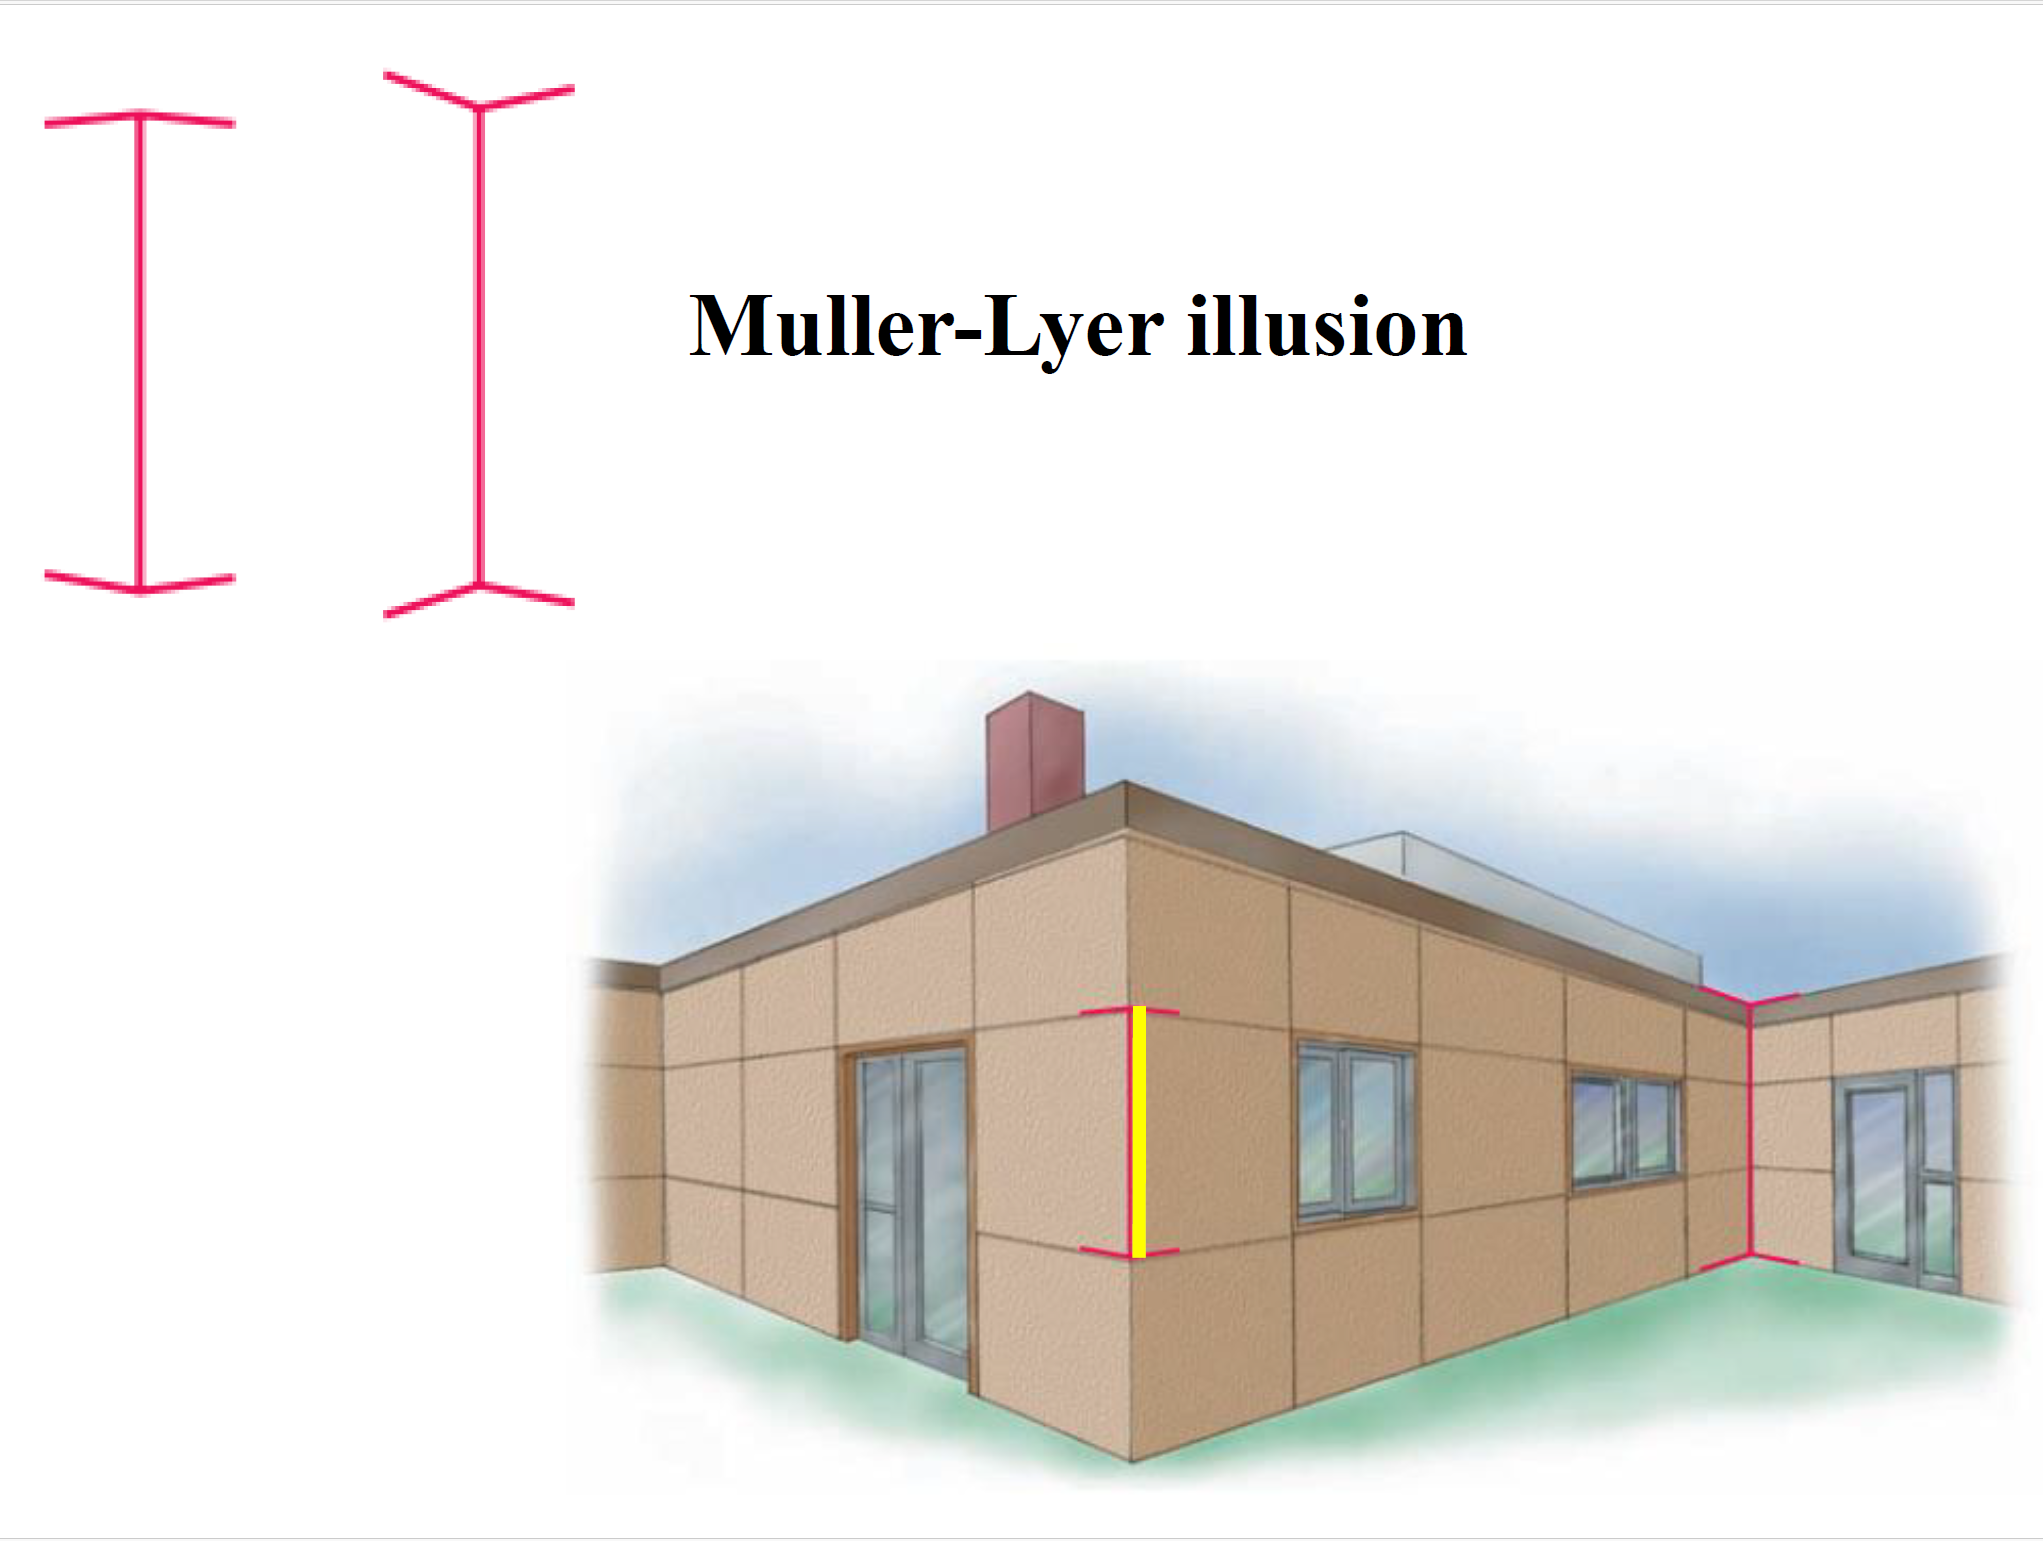
\includegraphics[width=0.65\columnwidth,height=0.45\linewidth]{Muller-Lyer_illusion}
    	\caption{Müller-Lyer illusion}
	\end{figure}

	对于这种错觉现象,有很多种解释。其中一种视角解释认为,
	我们的视觉系统会将直线的末端作为远处的角度或距离线索。
	因为我们对于远处的物体,末端向内凹的形状通常表示物体的
	角度向我们远离,而末端向外凸的形状表示物体的角度向我们
	靠近。因此,我们会错误地感知到有向内凹的直线更长。

	也就是说,此时对于我们的大脑而言,对于这个线段长度的
	合理推断(符合我们日常的经验和直觉),比它的真实长度更重要。

	\subsection{Beuchet Chair Illusion}
	当距离线索错误时,人们可能会产生一种错觉,称为Beuchet椅
	子错觉。这个错觉是由于我们对物体的距离和大小的感知存在
	偏差而引起的。

	Beuchet椅子错觉是通过对观察者造成视角误导引起的。
	一个人“坐在椅子上”,通过调整观察的视角,使从某个视角
	看上去,真实的椅子腿和那个人坐的“椅子的凳面”刚好拼接成了
	一个完整的椅子。

	实际上,我们对物体大小和距离的感知是通过多种线索来确定的,
	包括视角、线性透视和遮挡。当这些线索最后拼接而成的信息出现
	“差错”时,我们的大脑更倾向于使其合理化,而非真实情况。
	例如,在下图中,即使与我们的日常经验相悖,我们还是更倾向于
	相信这个人是站在椅子上的。为了合理解释这个现象,我们认为这
	个椅子的尺寸比正常情况大。
	\begin{figure}[h]
		\centering
    	\includegraphics[width=0.9\columnwidth,height=0.6\linewidth]{Beuchet Chair Illusion}
    	\caption{Beuchet Chair Illusion}
	\end{figure}

	\section{情绪}
	\subsection{定义}
	情绪是一种主观的体验,它可以受到多种因素的影响,包括个体的认知、
	解释和评估。人类大脑在处理情绪时,往往更关注情绪的合理性,即情绪
	体验是否与个体对于情境的解释和评估相一致。

	例如,当面临一种挑战性的情境时,个体可能会感到紧张和焦虑。然而,
	人类大脑更倾向于寻找合理的解释和理解,以帮助个体应对情境并调节情
	绪。个体可能会告诉自己,这种紧张和焦虑是正常的反应,它们可以提供
	动力和专注力,以应对挑战并取得成功。这种合理的解释和理解可以帮助
	个体调节情绪,使其更适应情境。

	因此,“对于人类的大脑而言,合理比真实更重要”,在情绪方面可以理解
	为人类大脑更注重情绪的合理解释和理解,以帮助个体应对情境并调节情
	绪。这强调了个体对情绪的主观解释和评估的重要性,而不仅仅依赖于情
	绪的客观真实性。

	\subsection{Dutton \texorpdfstring{\&}{} Aron, 1974 吊桥实验}
	实验中,研究人员邀请了一些男性参与者通过两座桥,一座是木桥,
	一座是吊桥。在通过这两座桥之前,他们会与一位女性研究员对话,对话
	结束后,女性研究员会给他们留下联系方式。表示如果对她的研究感兴趣的话,
	欢迎随时联系。

	结果显示,与对照组相比,实验组的参与者在过桥时表现出更强烈的情
	感和心理激活。他们的心率增加,呼吸加快,并且更有可能主动联系女
	性研究员。

	\begin{figure}[h]
		\centering
    	\includegraphics[width=0.9\columnwidth,height=0.5\linewidth]{Dutton & Aron, 1974 吊桥实验}
    	\caption{Dutton \& Aron, 1974 吊桥实验}
	\end{figure}

	实际情况是,在过吊桥时,实验者本身就感到紧张,导致他们心率增加、
	呼吸增加。但是因为实验组的实验者与女性研究员进行了短暂的对话,
	他们的大脑做出了合理的推断:自己心率加快、呼吸加快是因为对女性
	研究员产生了好感。

	\section{结语}

	综上所述,对于人类的大脑而言,合理比真实更重要。从大脑的结构和
	思考方式来看,我们的大脑在感知和知觉形成过程中会进行合理的推断,
	以形成知觉,而知觉结果可能与感觉的物理输入存在差别。在错觉方面,
	Müller-Lyer illusion和Beuchet Chair Illusion的例子表明,大
	脑会根据部分信息、经验和知识自动脑补出“合理”的结果,而可能与真
	实情况相悖。在情绪方面,Dutton \& Aron的吊桥实验显示,大脑更
	注重情绪的合理解释和理解,以帮助个体应对情境并调节情绪。因此,
	个体对于情绪的主观解释和评估的合理性比情绪的客观真实性更重要。
	
\end{document} 